% !Mode:: "TeX:UTF-8"
% !TEX program  = xelatex
\documentclass[a4paper]{IEEEtran}
\IEEEoverridecommandlockouts
\usepackage{ctex}
\usepackage{cite}
\usepackage{amsmath,amssymb,amsfonts}
\usepackage{algorithmic}
\usepackage{graphicx}
\usepackage{textcomp}
\usepackage{xcolor}
\usepackage[colorlinks,linkcolor=blue]{hyperref}
\usepackage[a4paper, top=2.54cm, bottom=2.54cm, left=3.18cm, right=3.18cm]{geometry}
\title{\huge{关于2017年以来\\
	本科毕业生去向变化的调查}\\
	\Large{——以上海交通大学为例}
}
\author{第二组：王凯灵、王浩新、黄幸运、刘明泽}
\begin{document}
	\maketitle
	\begin{abstract}
		当今社会出现了大学生就业困难、高等教育内耗严重等热点问题。对此，本文提出了一种关于近年来本科毕业生去向变化的调查方法，并且给出了一种基于所收集数据的大学生未来毕业去向和变化的预测方法，以期为解决解决该类问题提供指导性建议。
	\par\textbf{关键词—}
		毕业生、考研、就业、毕业去向、机器学习、Markov chain
	\end{abstract}

	\section{引言和研究背景：\\复杂的环境下大学生去向改变现象}
		当下，我国大学生毕业去向受到多方面因素影响：中美关系激化和贸易摩擦、2019年以来的新冠疫情冲击导致的经济问题和劳动力市场紧缩、周边战争的影响，变化较以前更加迅速。尤其是从2017年以来，我国考研人数增速明显加快。如图1所示$^{[1]}$，2022年考研人数较2017年已超过两倍。
	
		\begin{figure}[h]
			\centering
			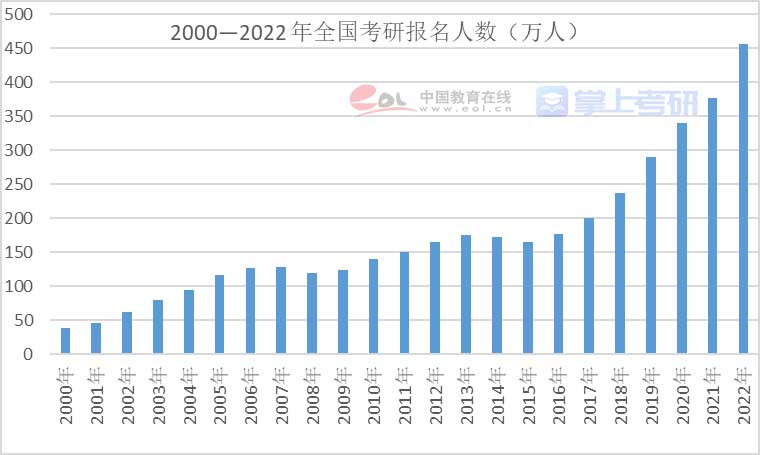
\includegraphics[width=0.9\linewidth]{研究生人数}
			\caption{2000年以来考研人数}
		\end{figure}
	
		同时，根据国家统计局给出的数据，2021年我国城镇就业人员减少约500万人，劳动力市场和人才市场都发生紧缩，推测大学生就业率相应下滑。限于疫情与国际关系，[1]中指出，我国留学人数也发生下滑现象。大学本科生毕业变化情况越来越引发人们关注。
		
		\section{研究综述：\\各类变化文献整理与以往研究不足}
			由于我们的研究的问题具有特定的时代背景，以往研究数量不多。以往研究显示，近年以来，疫情因素为大学生带来了更大的就业压力和心理压力，导致大学生陷入就业困难$^{[2]}$。疫情期间，国内经济情况不容乐观$^{[3]}$，人才市场和劳动力市场需求量减少$^{[4]}$，使得大学生更多的转向考研$^{[1]}$和考虑留学。而高等教育逆全球化现象也导致更多本可以出国留学的本科生加入考研队伍$^{[5]}$。由于疫情期间我国高等教育中线上教学较为普遍，网课教育对于人才质量的影响、疫情导致的线上面试求职方式也导致大学生就业困难$^{[3][5]}$。
			
			然而，以往研究主要关注了单一维度变化情况，如单独分析就业、考研等，并没有指明大学生毕业去向结构具体发生了何种变化及其原因。本研究致力于弥补这一缺失，多维度地分析本科生去向结构变化。
			
		\section{项目预期与价值：\\解决人才供求矛盾与资源内耗}
		\subsection{背景及研究价值}
		本次研究旨在把握当下受到疫情冲击的大学生就业及升学形势，探寻其面临的主要问题及成因，为该群体的学习和未来职业规划提供可供参考的信息和建议，有助干他们更好地规划自己的未来，平稳地由校园步入社会，同时也为相关政策的出台及完盖提供参考依据，建言献策，对于暂时未面临就业及升学问题的大一和大二学生，本次研究也将其纳入研究对象，以期通过兼顾低年级学生获得更为全面客观的分析。
		\subsection{预期成果}
		通过本次课题研究，我们希望得到近5年以来本科生毕业去向的具体数据及其类间变化，预测未来变化走向。同时探究本科生毕业去向发生变化的可能原因，并得出对于政府部门、人才市场和应届毕业生的发展和规划建议。
		通过得到的数据，我们会向相关部门提供建议，帮助国内人力资源市场快速复苏，缓解人才供求矛盾与高等教育内耗，并预测本科生毕业去向未来变化，为应届生和人力资源部门提供提前规划的参考，最终实现最大化人才资源利用率。
		\section{项目流程：\\预调研-问卷-访谈三步式研究设计}
		在本研究项目中，我们的研究过程主要分为三个部分：预访谈、问卷调查和正式访谈。在问卷调查中，我们希望得到各届毕业生的预期去向以及实际去向的实际数据，并且与校方的可靠档案进行对照，而在访谈中我们将探究毕业生近几年毕业去向产生变化的具体原因。
		\subsection{样本选取}
		首先我们需要确定我们研究的样本范围。在本项目中我们希望能够考虑到疫情因素对大学生就业去向选择产生的影响，因此我们的研究对象需要覆盖疫情前后毕业的多届学生以便进行对比。在这里，我们初步选择2017-2022届交大本科毕业生。2017届到2019届的毕业去生向完全不受到疫情影响，而2020到2022届毕业生则是受到疫情影响较为严重的部分。再进一步，我们还可以考虑选择2023届及之后毕业的受疫情影响相对较轻的在校生进行调研，并同之前的数据进行对比增强我们研究的说服力。考虑到各个专业的去向差异比较大，在样本的选取时需要尽量保证各个专业和重点学科的样本数占该专业总人数的比例大致相同。由于交大近年来招生人数较为稳定，我们还要保证各届毕业生的人数相当。对于出国留学和就业创业的毕业生可能难以联系，我们还需要将数据同校方档案进行比较，专项补齐这些缺失的内容。
		\subsection{预访谈设计}
		确定样本范围之后我们就可以参考前人的研究内容进行预访谈的设计。在预访谈中，我们的主要目标是大致了解各界毕业生就业去向的基本情况以及一些可能会影响去向选择的因素，并通过这些信息设计出较为合理的调研问卷和深度访谈内容。首先我们需要了解该毕业生的专业、毕业时间和去向以及当时的基本形势等让我们能够对该样本进行简单的分类。我们还需要了解其毕业前的预期去向，如果实际去向与预期去向不符合则需要探究产生变化的原因，如果是一致的则考察是什么因素推动了这种选择。如果该毕业生是疫情后毕业的则需要重点关注其疫情前后的预期以及疫情因素对去向的选择产生了多大的影响。
		\subsection{问卷设计}
		在了解了基本信息之后就可以通过问卷获得毕业生去向的具体数据。在这个部分中我们希望得到毕业前的预期去向和实际去向的数据。对经历过疫情的毕业生则需要进一步的考察其在疫情前后预期方向的变化以及产生这种变化的原因，包括国际冲突加剧、疫情引起的经济衰退和健康安全考虑等，由预访谈的结果具体考虑。通过对比不同年级不同专业的去向数据我们可以大致了解近年毕业生去向的变化情况。
		\subsection{深度访谈与案例研究}
		最后，结合预访谈和问卷调研获得的数据我们进一步设计深度访谈，探究毕业去向变化的具体原因。除了和预访谈相同的内容外，在深度访谈中，我们需要更多的关注每一年就业升学市场的具体形势、疫情对毕业生的冲击以及毕业生预期去向产生变化的心路历程。
		\section{数据处理}
		以往研究也有使用机器学习方法对大学生毕业去向进行预测，比如使用Lasso-逻辑回归方法从大学生身份信息推测大学生毕业去向，取得了70\%以上的准确率$^{[6]}$，也有使用灰色系统模型预测大学生就业率的方法$^{[7]}$，准确率高达96.38\%。在我们的研究中，由于我们收集的数据量小，时间上顺序相关，可以认为是离散时间序列预测任务，可以使用隐马尔科夫链进行数学建模。
		\subsection{变量规定}
		我们通过问卷可以得到的所需信息是：大学生期望去向、在提前一年毕业的假设下大学生毕业预期去向。我们仅使用三个主要去向：就业、读研、留学。
		
		我们定义：
		\begin{itemize}
		\item 状态转移率
		$$
		\mathrm{Ts}(\mathrm{a}, \mathrm{b})=\frac{\mathrm{a} \text { 转入 } \mathrm{b}}{\mathrm{a} \text { 总数 }}
		$$

		\item 状态转移矩阵
		$$\boldsymbol{T}=
		\left(\begin{array}{lll}
			\operatorname{Ts}(1,1) & \operatorname{Ts}(1,2) & \operatorname{Ts}(1,3) \\
			\operatorname{Ts}(2,1) & \operatorname{Ts}(2,2) & \operatorname{Ts}(2,3) \\
			\operatorname{Ts}(3,1) & \operatorname{Ts}(3,2) & \operatorname{Ts}(3,3)
		\end{array}\right)
		$$
		如图2所示。
		
		\begin{figure}[h]
			\centering
			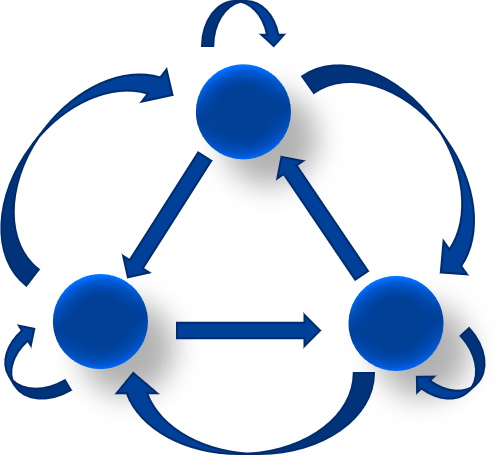
\includegraphics[width=0.7\linewidth]{转移矩阵}
			\caption{状态转移}
		\end{figure}
		\end{itemize}
		\subsection{基本假设}
		使用马尔可夫关系存在简单假设：下一个状态的情况仅仅依赖于上一个状态，在实际问题中，我们近似的认为：
		\begin{itemize}
			\item 下一届的毕业生的主要参考对象是上一届的毕业生。
			\item 两年间社会环境不会发生突变。
		\end{itemize}
		事实上，由于下文的计算使用多年间的平均情况，所以第二个假设虽然不够合理，但不会造成显著影响。
		\subsection{预测方法}
		通过收集的提前假设下预期去向，我们可以得到状态转移矩阵的观测值$\boldsymbol{\hat T}$. 根据连续四年的数据，应用马尔科夫关系，我们可以列写方程完全解出适用于这四年间的状态转移矩阵，如图3所示。我们不妨用该矩阵代替其中间2年的转移矩阵，可以起对比验证作用。
		\begin{figure}[h]
			\centering
			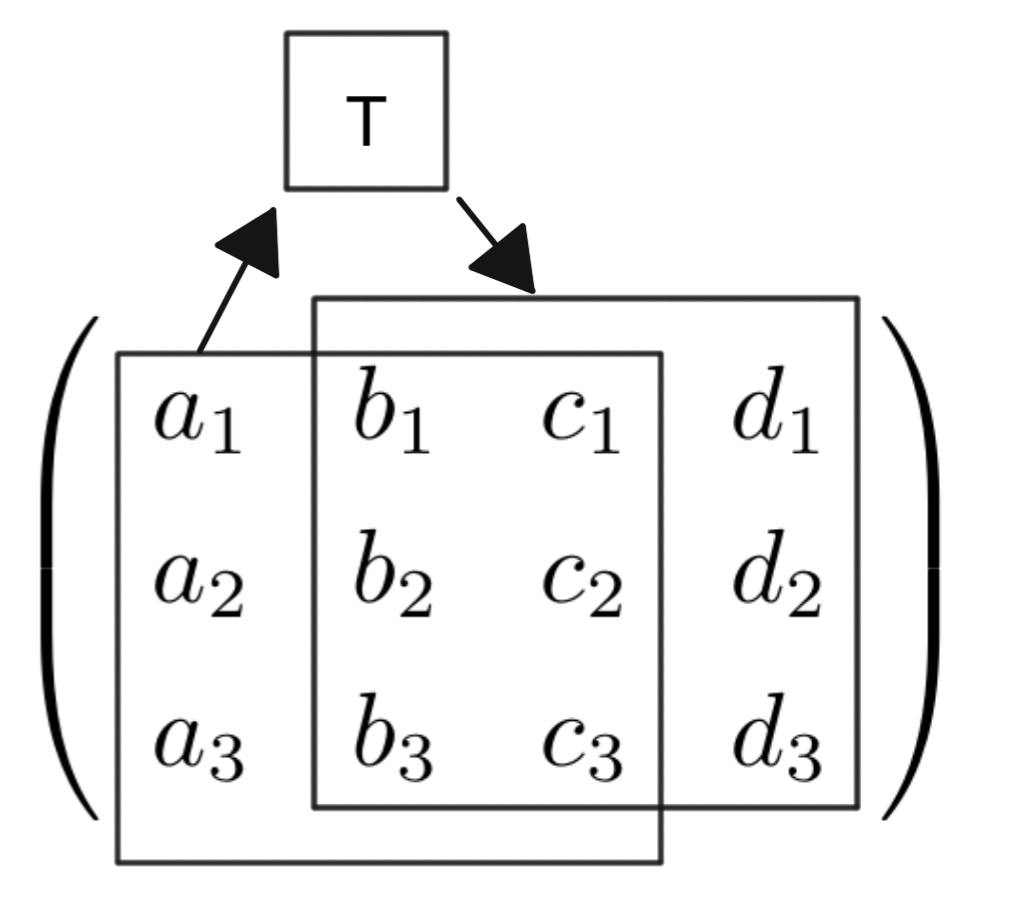
\includegraphics[width=0.7\linewidth]{计算}
			\caption{隐藏状态转移矩阵}
		\end{figure}
		
		由于我们的数学模型中，状态转移矩阵不断变化，所以我们对转移矩阵本身再次使用马尔科夫关系。我们希望得到的转移矩阵是数据最后三年向未来一年的转移矩阵。我们通过转移矩阵构成的马尔科夫链向后拟合，使用这三年数据的两次转移关系模拟得到该矩阵。最后一年的数据乘以改矩阵得到未来一年数据，即达到预测目的。
		\section{反思与总结}
		我们组进行的调研是关于2017年以来本科毕业生去向变化的调查。在国际争端不断，疫情形势复杂，经济走向不乐观等多种因素综合影响下，本科生的升学受到了很大的影响，最明显的就是考研人数激增。本调研探究本科生毕业去向发生变化的可能原因，有助于得出对于政府部门、人才市场和应届毕业生的发展和规划建议，最终实现最大化人才资源利用率。
		
		通过对已有文献的阅读发现，以往的研究更多关注大学生群体的单一去向的变化趋势，如留学率、就业率等，未有对不同去向间变化趋势及其原因的研究。因而我们希望得到近5年以来本科生毕业去向的具体数据及其类间变化，预测未来变化走向。
		
		在研究方案上，我们选择在2017-2022届交大本科生（抽样）里进行抽样调查。这有利于提高收集、整理数据、综合样本的速度，保证调查的时效性，同时也能更准确地推算出交大本科生的总体趋势。在选取样本上，我们进行了一定的处理，以降低误差：
		\begin{enumerate}
			\item 使得各届人数基本相同
			\item 学院与重点专业分布归一化
			\item 与校方存档数据进行比较
		\end{enumerate}
		
		在方案流程上，我们设定了预调研，问卷调查，深入访谈三个步骤，在流程上环环相扣，以期使问题的设计更准确，贴合实际，获得的数据更真实，价值更大。
		
		在预调研中，我们首先进行先前研究，在既有资料上设计访谈问题，再通过预防谈的样例来了解大致情况，决定问卷设计，设计深度访谈，从而改进已有的方案。
		
		之后，我们以有偿问卷的形式，希望获得更真实，更准确，更优质的数据。预期获得2万份调查样本，从中收集毕业生的预期去向和实际去向，并比较二者的差异。
		
		最后，我们将进行深入访谈。我们将访谈目标分为3类不同去向的人群和9种不同变化的群体。在已有的文献资料和前期数据获取与分析的基础上，我们希望设计更好的问题，进行案例研究，以深度挖掘变化原因，进行深度访谈，发掘更深刻的社会问题。
		
		同时，为了使数据更准确，更真实，更能反应总体趋势而达到预期效果，我们结合专业所学知识进行数据处理：首先，进行数据清洗，处理掉无效数据。之后，量化关系，设计公式计算。这里我们考虑使用马尔科夫链，通关计算状态转移率和状态转移矩阵，进行数据的计算和趋势的预测。最后，进行数据分析并得出结论。
		
		\section{缺陷分析}
		尽管我们的方案已经尽可能地考虑周全，但是经过后期的讨论，我们仍发现有一定的缺陷。例如，众所周知，不同专业间存在着一定的就业情况差异，计算机科学与技术和仪器科学与技术专业就业情况就显著不同，我们应该如何解决？不同专业年龄差异是否会造成影响？创业人员、出国人员可能难以取得联系，问卷样本是否可能出现偏差？研究的是变化，直接比较去向记录即可得到，为何需要问卷？经过分析，我们的解决方案如下。对于专业差异问题，我们保证各专业比例构成基本一致，使数据结构更加合理，必要时可以单独分析部分专业情况。而对于年龄差异的问题，我们可以考虑每年调查一个年级，以消除此差异。而对于一些难以取得联系的人员，我们将与校方记录进行比较，如有此情况可动用人员单独联系和通过案例研究弥补。而对于最后一个问题，我们认为，去向意向变化体现为实际变化，具有滞后性，比如考研人数激增不会导致录取人数随之增加。研究去向意向的变化对于解决实际社会问题更具有价值和指导意义。
		
		在调研结束之后，经过客观的评价与理性的分析，我们发现我们虽然具有不足之处，但仍争取做到尽可能地减小误差，完善方案，并尝试着结合专业知识来解决问题。
		
		\section{小组分工}
		\begin{itemize}
			\item 王凯灵(组长):负责了研究路线方案设计、研究逻辑陈述思路设计、PPT制作和展示、问卷访谈内容补充。报告部分负责了研究综述及之前部分、数据处理部分和排版。此外提供了预测代码简单实现。
			\item 王浩新：负责了前期文献收集和调研、合作完成了访谈设计和模拟访谈记录。报告部分完成了反思与总结、缺陷分析部分，原文见附件。
			\item 黄幸运：负责了前期文献收集和调研、完成与问卷内容文字部分、参与模拟访谈。报告部分负责了方案流程部分，原文见附件。
			\item 刘明泽：研究问题提出者、负责了前期文献收集和调研、完成问卷制作。报告部分负责了项目预期与价值部分、背景部分，原文见附件。
		\end{itemize}
		\section{课程认识与收获}
		\begin{itemize}
			\item 王凯灵：通过本课程，我发现社会科学在某一些问题上可以与我个人的专业方向展开合作，实现社会科学研究方法上的创新。同时，在和老师不断交流中，我感受到老师和我共同进步。关于蜘蛛听觉器官在脚上的例子，我是从浙江大学出版的高中生物读本上读到的，在生物研究方法模块作者引用该例子增加读本趣味性。也因此，我进一步认识到了学科之间的无限交叉。
			\item 王浩新：社会科学研究方法这门课对我来说意义很大。一方面，我了解了文献对学术研究的价值，学会了如何去通过各大平台搜索文献，如何去辨识文献，找到我所需要的资料，这对我们以后的工作无疑是有重要作用的。另一方面，我也了解了关于调研的一些知识，诸如变量，问卷和访谈的联系与区别等等，知道了调研需要注意的一些细节以及调研有哪些方法。最后，我们通过期末作业的形式付诸于实践，更深刻地理解了调研的意义，同时也能更好地运用所学的方法，成功做到了理论用于实践。
			\item 黄幸运：学习这门课程最主要的收获还是学习到了社会科学研究的一些相关方法。作为理科学生平时接触的都是理工科，很少关注社会科学。通过这门课程的学习首先是了解了一下文献查阅方面的技巧，这类技巧是无论做什么科学研究都通用的，非常有效。其次就是了解了一些社会科学方面的研究方法，也许之后能够为理工科的研究提供一些新的思路，也能够拓展我们的思维。
			\item 刘明泽：学习社会学研究方法对于我来说真的有很大的帮助，长远的不说，就在学校科研立项、特色调研、暑期调研等活动的开展过程中，社会学研究方法起着非常重要的作用。半个学期下来，我对于如何选题、如何制定研究方案、设计调查问卷、如何进行测量与数据分析、以及如何进行访谈等社会学研究的各个环节有了更深入的了解。最后我参与的小组项目动手实践设计问卷，大概体验了社会科学研究项目从提出到设计的过程。
		\end{itemize}
	\section{参考文献}
	[1]~\href{https://www.eol.cn/e_ky/zt/report/2022/index.html}{2022年全国研究生调查报告. 中国教育在线}
	
	[2]李春玲.疫情冲击下的大学生就业:就业压力、心理压力与就业选择变化[J].教育研究,2020,41(07):4-16.
	
	[3]朱武祥,张平,李鹏飞,王子阳.疫情冲击下中小微企业困境与政策效率提升——基于两次全国问卷调查的分析[J].管理世界,2020,36(04):13-26.DOI:10.19744/j.cnki.11-1235/f.2020.0049.
	
	[4]沈国兵.“新冠肺炎”疫情对我国外贸和就业的冲击及纾困举措[J].上海对外经贸大学学报,2020,27(02):16-25.DOI:10.16060/j.cnki.issn2095-8072.2020.02.002.
	
	[5]钟秉林,南晓鹏.后疫情时代我国高等教育发展的宏观思考[J].教育研究,2021,42(05):108-116.
	
	[6]亓红强,张福堃,高大鲲,王惠强.基于灰色系统的大学生就业率预测[J].现代电子技术,2019,42(11):174-177.DOI:10.16652/j.issn.1004-373x.2019.11.040.
	
	[7]孙怡帆,潘昆峰,孙正阳,何章立.大学生毕业去向预测的思路与方法——基于机器学习算法的尝试[J].教育学术月刊,2019(01):25-35.DOI:10.16477/j.cnki.issn1674-2311.2019.01.003.
	
\end{document}